% Sección 15.7: Aplicaciones de las Ecuaciones Diferenciales de Segundo Orden

Las ecuaciones diferenciales lineales de segundo orden tienen una variedad de aplicaciones en las ciencias e ingeniería. En esta sección se exploran dos de ellas: vibración de resortes y circuitos eléctricos.

\subsection*{Resortes Vibratorios}

Se considera el movimiento de un objeto de masa $m$ sujeto al extremo de un resorte que es ya sea vertical (como en la figura 15.8) u horizontal sobre una superficie plana (como en la figura 15.9).

En la sección 5.4 se consideró la ley de Hooke, la cual establece que si el resorte es estirado (o comprimido) $x$ unidades con respecto a su longitud natural, entonces ejercerá una fuerza proporcional a $x$:
\[ \text{fuerza de recuperación} = -kx \]

\vspace{0.5cm}
\begin{center}
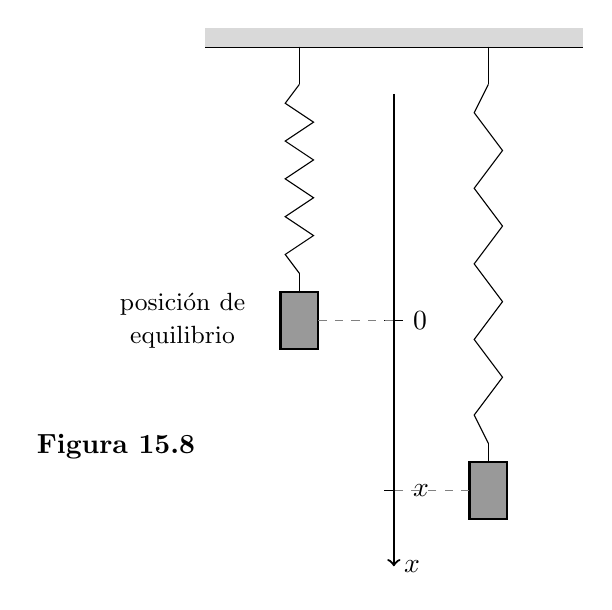
\begin{tikzpicture}[scale=1.2]
    % Soporte superior (Techo)
    \draw[thick] (-2, 4) -- (2, 4);
    \fill[gray!30] (-2, 4) rectangle (2, 4.2);

    % PRIMER RESORTE (Posición de equilibrio)
    \draw (-1, 4) -- (-1, 3.6);
    % Zigzag manual para evitar dependencias de librerías extra
    \draw (-1, 3.6) -- (-1.15, 3.4) -- (-0.85, 3.2) -- (-1.15, 3.0) -- (-0.85, 2.8) -- (-1.15, 2.6) -- (-0.85, 2.4) -- (-1.15, 2.2) -- (-0.85, 2.0) -- (-1.15, 1.8) -- (-1, 1.6);
    \draw (-1, 1.6) -- (-1, 1.4);
    % Masa
    \filldraw[fill=gray!80, draw=black, thick] (-1.2, 0.8) rectangle (-0.8, 1.4);

    % SEGUNDO RESORTE (Estirado a la posición x)
    \draw (1, 4) -- (1, 3.6);
    % Zigzag más estirado
    \draw (1, 3.6) -- (0.85, 3.3) -- (1.15, 2.9) -- (0.85, 2.5) -- (1.15, 2.1) -- (0.85, 1.7) -- (1.15, 1.3) -- (0.85, 0.9) -- (1.15, 0.5) -- (0.85, 0.1) -- (1, -0.2);
    \draw (1, -0.2) -- (1, -0.4);
    % Masa estirada
    \filldraw[fill=gray!80, draw=black, thick] (0.8, -1.0) rectangle (1.2, -0.4);

    % EJE VERTICAL (x)
    \draw[->, thick] (0, 3.5) -- (0, -1.5) node[right] {$x$};
    
    % Marca de equilibrio (0)
    \draw (-0.1, 1.1) -- (0.1, 1.1) node[right] {$0$};
    \draw[dashed, gray] (-0.8, 1.1) -- (0, 1.1);
    \node[left, align=center, text width=2cm] at (-1.3, 1.1) {\small posición de \\ equilibrio};
    
    % Marca de estiramiento (x)
    \draw (-0.1, -0.7) -- (0.1, -0.7) node[right] {$x$};
    \draw[dashed, gray] (0.8, -0.7) -- (0, -0.7);

    % Etiqueta de la figura
    \node[below left] at (-2, 0) {\textbf{Figura 15.8}};
\end{tikzpicture}
\end{center}

También se pueden transferir otras ideas de una situación a otra. Por ejemplo, la solución estacionaria considerada en la nota 1 tiene interpretación en el sistema resorte-masa. Y el fenómeno de resonancia en el sistema resorte-masa se puede llevar en forma útil a los circuitos eléctricos en forma de resonancia eléctrica.

\begin{table}[h]
\centering
\begin{tabular}{ll|ll}
\hline
\multicolumn{2}{c|}{\textbf{Sistema Resorte-Masa}} & \multicolumn{2}{c}{\textbf{Circuito Eléctrico}} \\ \hline
$m$ & masa & $L$ & inductancia \\
$c$ & constante de amortiguación & $R$ & resistencia \\
$k$ & constante del resorte & $1/C$ & elastancia \\
$F(t)$ & fuerza externa & $E(t)$ & fuerza electromotriz \\
$dx/dt$ & velocidad & $I = dQ/dt$ & corriente \\ \hline
\end{tabular}
\end{table}

\subsection*{Ejercicios 1--6: Problemas aplicados de oscilación mecánica (Sistema Resorte-Masa), amortiguación crítica y sobreamortiguación.}
\begin{enumerate}
    \subimport{ejercicio_01/}{ejercicio.tex}
    \subimport{ejercicio_02/}{ejercicio.tex}
    \subimport{ejercicio_03/}{ejercicio.tex}
    \subimport{ejercicio_04/}{ejercicio.tex}
    \subimport{ejercicio_05/}{ejercicio.tex}
    \subimport{ejercicio_06/}{ejercicio.tex}
\end{enumerate}

\subsection*{Ejercicios 7--8: Demostraciones analíticas de oscilaciones forzadas y resonancia pura por coeficientes indeterminados.}
\begin{enumerate}
    \setcounter{enumi}{6}
    \subimport{ejercicio_07/}{ejercicio.tex}
    \subimport{ejercicio_08/}{ejercicio.tex}
\end{enumerate}

\subsection*{Ejercicios 9--12: Circuitos eléctricos en serie RLC con baterías constantes y generadores de voltaje alterno.}
\begin{enumerate}
    \setcounter{enumi}{8}
    \subimport{ejercicio_09/}{ejercicio.tex}
    \subimport{ejercicio_10/}{ejercicio.tex}
    \subimport{ejercicio_11/}{ejercicio.tex}
    \subimport{ejercicio_12/}{ejercicio.tex}
\end{enumerate}

\subsection*{Ejercicio 13: Demostración analítica de la forma de fase de amplitud para oscilaciones armónicas libres.}
\begin{enumerate}
    \setcounter{enumi}{12}
    \subimport{ejercicio_13/}{ejercicio.tex}
\end{enumerate}
